\documentclass[a4paper,14pt]{article}
\usepackage[a4paper, mag=1000, left=2.5cm, right=1cm, top=2cm, bottom=2cm, headsep=0.7cm, footskip=1cm]{geometry}
\usepackage[utf8]{inputenc}
\usepackage[T2A]{fontenc}
\usepackage[english,russian]{babel}
\usepackage{indentfirst}
%\usepackage[dvipsnames]{xcolor}
\usepackage[colorlinks]{hyperref}
\usepackage{amsfonts} 
\usepackage{amsmath}
\usepackage{graphicx}
\usepackage{float}

\DeclareGraphicsExtensions{.png,.jpg}

\usepackage{fancyhdr}
\pagestyle{fancy}
\fancyhead[LE,RO]{\thepage}
\fancyfoot{}

\usepackage{listings}

\hypersetup{linkcolor=black}

\title{non-linear equations}
\author{Иван Золин}
\date{2023}
\thispagestyle{empty}
\begin{document}
	
	\begin{titlepage}
		\begin{center}
			\textsc{
				Санкт-Петербургский политехнический университет имени Петра Великого \\[5mm]
				Физико-механический институт\\[2mm]
				Высшая школа прикладной математики и физики            
			}   
			\vfill
			\textbf{\large
				Интервальный анализ\\
				Отчёт по лабораторной работе №2 \\[3mm]
			}                
		\end{center}
		
		\vfill
		\hfill
		\begin{minipage}{0.5\textwidth}
			Выполнил: \\[2mm]   
			Студент: Золин Иван \\
			Группа: 5030102/00201\\
		\end{minipage}
		
		\hfill
		\begin{minipage}{0.5\textwidth}
			Принял: \\[2mm]
			к. ф.-м. н., доцент \\   
			Баженов Александр Николаевич
		\end{minipage}
		
		\vfill
		\begin{center}
			Санкт-Петербург \\2023 г.
		\end{center}
	\end{titlepage}
	
	\tableofcontents
	\newpage
	
	\section{Постановка задачи}
	Имеем ИСЛАУ:
	\begin{equation*}
		\begin{cases}
			[2, 4]*x_1 + [4,6]*x_2 = [5, 9]\\
			3*x_1 + [-6, -4]*x_2 = [-1, 1]\\
			[0.5, 1.5]*x_1 = [1, 3]\\
			[0.5, 1.5]*x_2 = [0, 2]\\
		\end{cases}
	\end{equation*}
	Необходимо найти решения ЛЗД. Для этого нужно
	\begin{itemize}
		\item исследовать разрешимость ЛЗД (найти максимум распознающего функционала)
		\item коррекция ЛЗД
		\begin{itemize}
			\item достижение разрешимости ИСЛАУ за счет коррекции правой части (равномерное/неравномерное)
			\item достижение разрешимости ИСЛАУ за счет коррекции матрицы
		\end{itemize}
	\end{itemize}
	\section{Теория}
	\subsection{Распознающий функционал}
	Разпознающим функционалом называется функция
	\begin{equation}
		\mathrm{Tol}(x)=\mathrm{Tol}(x,\mathbf{A},\mathbf{b})=\min_{1\leq i\leq m}\left\{\mathrm{rad}(\mathbf{b}_i)-\left|\mathrm{mid}(\mathbf{b}_i)-\sum_{j=1}^n \mathbf{a}_{ij}x_j\right|\right\}
	\end{equation}
	Пусть
	\begin{equation}
		T=\max_{x\in \mathbb{R}^n} \;\mathrm{Tol}(x, \mathbf{A},\mathbf{b})
	\end{equation}
	и это значение достигается распознающим функционалом в некоторой точке $\tau\in \mathbb{R}^n$. Тогда
	\begin{itemize}
		\item если $T\geq0$, то $\tau\in\Xi_{\mathrm{tol}}(\textbf{A},\textbf{b})\neq  \emptyset$, т.е. линейная задача о допусках для интервальной линейной системы $\textbf{A}x=\textbf{b}$ совместна и точка $\tau$ лежит в допусковом множестве решений.
		\item если $T>0$ то $\tau\in int \;\Xi_{\mathrm{tol}}(\textbf{A},\textbf{b})\neq  \emptyset$, и принадлежность $\tau$ допусковому множеству решений устойчива к малым возмущениям данных - матрицы и правой части.
		\item если $T<0$ то $\Xi_{\mathrm{tol}}(\textbf{A},\textbf{b})=\emptyset$,  т.е. линейная задача о допусках для интервальной линейной системы $\textbf{A}x=\textbf{b}$ несовместна.
	\end{itemize}
	\subsection{Достижение разрешимости ИСЛАУ путём изменения правой части}
	\textbf{Равномерное уширение правой части
		ИСЛАУ}\\
	Расширение вектора $\textbf{b}$ происходит путем его замены на вектор: 
	\begin{equation}
		\textbf{b}+K\textbf{e}, \;\; K\geq 0, \;\; \textbf{e}=([-1, 1],...,[-1, 1])^T
	\end{equation}
	Тогда
	\begin{equation}
		\max_{x\in \mathbb{R}^n} \;\mathrm{Tol}(x, \mathbf{A},\mathbf{b}+K\textbf{e}) = T + K
	\end{equation}
	Но $\mathrm{Arg}\max\mathrm{Tol}$ - не изменится(положение точки Т) \\
	\\
	\textbf{Неравномерное уширение правой части
		ИСЛАУ}\\
	Если линейная задача о допусках с матрицей $\textbf{A}$ и вектором правой части $\textbf{b}$ первоначально не имела решений, то новая задача с той же матрицей  $\textbf{A}$ и уширенным вектором
	\begin{equation}
		(\textbf{b}_i+K\cdot v_i\cdot [-1,1])_{i=1}^m
	\end{equation}
	в правой части становится разрешимой при $K\geq |T_v|$, где
	\begin{equation}
		T_v=\min_{1\leq i\leq m}\left\{v_i^{-1}\left(\mathrm{rad}(\mathbf{b}_i)-\left|\mathrm{mid}(\mathbf{b}_i)-\sum_{j=1}^n \mathbf{a}_{ij}x_j\right|\right)\right\}
	\end{equation}
	Значение $\mathrm{Arg}\max\mathrm{Tol}$ -  изменится
	\subsection{Достижение разрешимости ИСЛАУ путём изменения матрицы}
	Общая схема равномерного метода заключается в том, что необходимо модифицировать матрицу $\textbf{A}$ засчет ее замены на $\mathbf{A}\ominus \mathbf{E}$, где 
	% $N = \{v_i\}$ - матрица весов $K$ - общий коэффициент сужения $\mathbf{A}, \; 
	$\mathbf{E}$ состоит из $\mathbf{e}_{ij}=[-e_{ij}, e_{ij}]$ \\
	Причем значения точечных величин $\mathbf{e}_{ij}$ удовлетворяют двум условиям:
	\begin{equation}
		0 \leq \mathbf{e}_{ij} \leq rad{\;\mathbf{a}_{ij}} \\
	\end{equation}
	\begin{equation}
		\sum_{j=1}^n e_{ij}\tau=K, \quad i=1,2,...,m, \quad K>0
	\end{equation}
	Если $K\geq |T|$, то тогда линейная задача о допусках с матрицей $\mathbf{A}\ominus\mathbf{E}=([\underline{\mathbf{a}}_{ij}-\underline{\mathbf{e}}_{ij},\overline{\mathbf{a}}_{ij}+\overline{\mathbf{e}}_{ij}])$ и правой частью $\textbf{b}$ становится разрешимой.
	\subsection{Оценки вариабельности решения}
	Абсолютной вариабельностью оценки называется величина
	\begin{equation}
		\mathrm{ive}(\mathbf{A},\mathbf{b})=\min\limits_{A\in\mathbf{A}}\mathrm{cond}\:A\cdot||\arg\max\:\mathrm{Tol}(x)||\frac{\max\limits_{x\in\mathbb{R}^n}\mathrm{Tol}(x)}{||\mathbf{b}||}
	\end{equation}
	Относительной вариабельностью оценки называется величина
	\begin{equation}
		\mathrm{rve}(\mathbf{A},\mathbf{b})=\min\limits_{A\in\mathbf{A}}\mathrm{cond}\:A\cdot\max\limits_{x\in\mathbb{R}^n}\mathrm{Tol}(x)
	\end{equation}
	\section{Реализация}
	\subsection{Описание}
	Данная лабораторная работа была выполнена с использованием языка
	программирования Python 3.10 в среде разработки Visual Studio Code.
	Используются библиотеки: numpy, intvalpy, matplotlib.
	Отчёт подготовлен с помощью языка LaTEX в редакторе TexStudio.
	\subsection{Ссылка на репозиторий}
	\url{https://github.com/IMZolin/Interval-analysis} \ - GitHub репозиторий
	
	\section{Результат}
	\subsection{Максимум распознающего функционала}
	\begin{figure}[H]
		\centering
		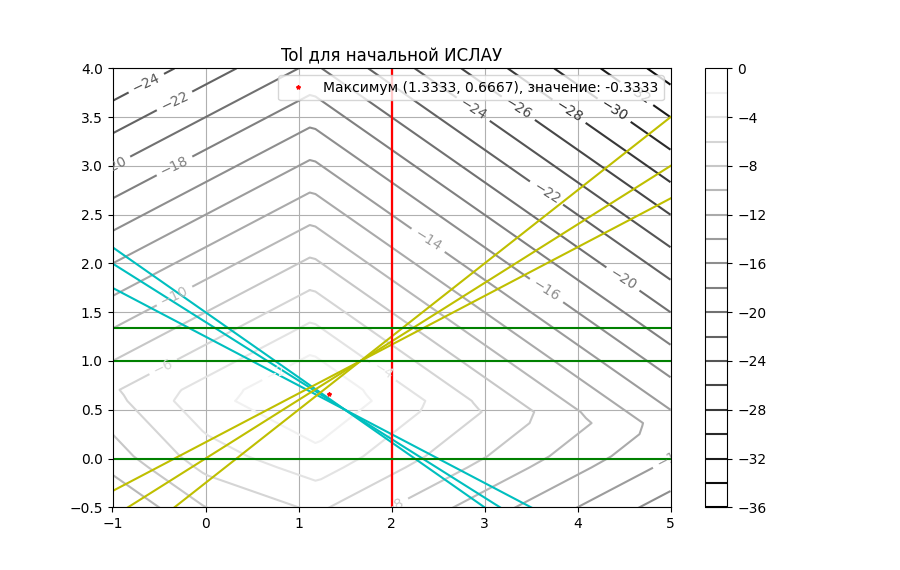
\includegraphics[width=0.7\textwidth]{../src/pic/Tol1.png}
		\caption{Расположение максимума распознающего функционала} 
	\end{figure}
	Максимум со значением $T=-0.333$ расположен в точке $\tau=(1.333,0.6667)$.
	\subsection{Достижение разрешимости за счёт коррекции правой части}
	\subsubsection{Равномерное уширение}
	Положим $K=1$. Получается максимум со значением $T=0.6667$ расположен в точке $\tau=(1.333,0.6667)$. При этом видим, что точка максимума осталась прежней.
	\begin{figure}[H] \label{MatrixCorrSet}
		\centering
		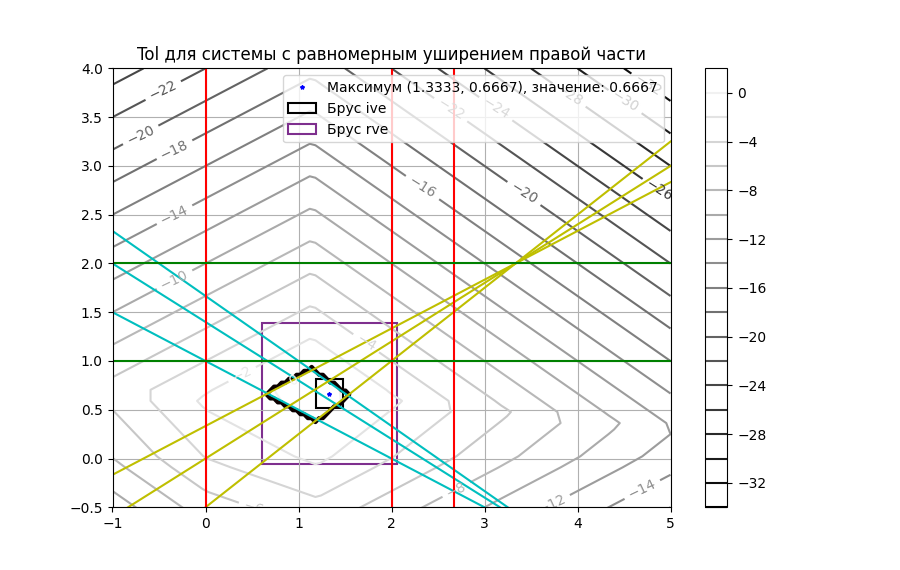
\includegraphics[width=0.7\textwidth]{../src/pic/even_right.png}
		\caption{Допусковое множество решений с равномерным уширением правой части} 
	\end{figure}
	\noindent На данном рисунке черный квадрат имеет сторону $2\cdot \mathrm{ive}$, а фиолетовый - $2\cdot \mathrm{rve}$. Область обведенная черной линией - допусковое множество\\
	$\mathrm{ive}: 0.1473502 \;\;\;\mathrm{rve}: 0.726363348$
	
	\subsubsection{Неравномерное уширение}
	Выберем произвольный вектор $v = [0.5, 0.1, 1, 0.5]$ и постоянную $K = 3$. \\
	Получается максимум со значением $T=0.724$ расположен в точке $\tau=(0.96, 0.576)$. При этом видим, что точка максимума сдвинулась.
	\begin{figure}[H] \label{MatrixCorrSet}
		\centering
		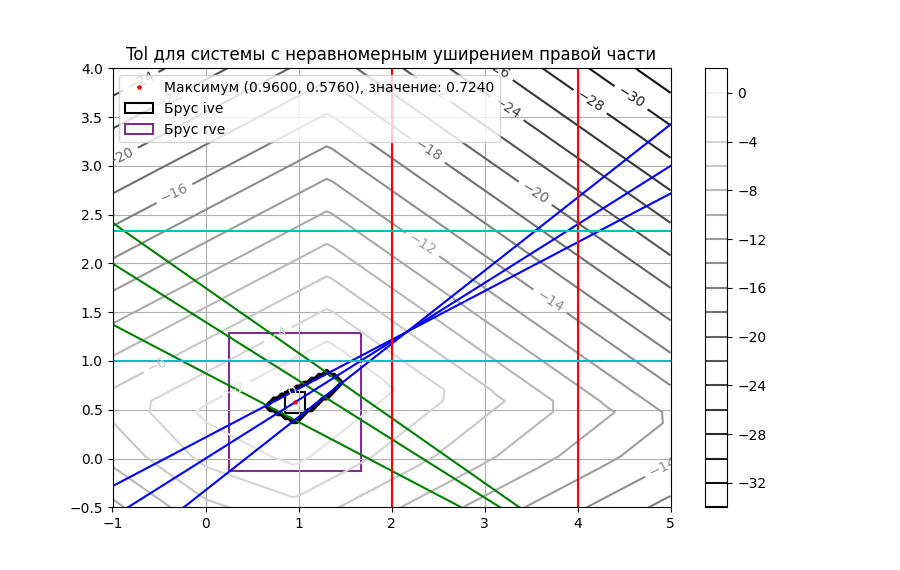
\includegraphics[width=0.7\textwidth]{../src/pic/uneven_right.png}
		\caption{Допусковое множество решений с неравномерным уширением правой части} 
	\end{figure}
	\noindent На данном рисунке черный квадрат имеет сторону $2\cdot \mathrm{ive}$, а фиолетовый - $2\cdot \mathrm{rve}$. Область обведенная черной линией - допусковое множество\\
	$\mathrm{ive}: 0.106272696 \;\;\;\mathrm{rve}: 0.69755409$
	
	\subsection{Достижение разрешимости за счёт коррекции левой части}
	Для построения интервальной матрицы $\textbf{E}$ с уравновешанными интервальными элементами $\mathbf{e}_{ij}=[-e_{ij}, e_{ij}]$ выбираем такие $\mathbf{e}_{ij}$, что:
	\begin{equation*}
		\begin{cases}
			0 \leq \mathbf{e} \leq 1 = \mathrm{rad}(\textbf{a}_{11}), \mathrm{rad}(\textbf{a}_{12}), \mathrm{rad}(\textbf{a}_{22}) \\
			0 \leq \mathbf{e} \leq 0.5 = \mathrm{rad}(\textbf{a}_{31}), \mathrm{rad}(\textbf{a}_{42}) \\
			1.333*\mathbf{e} + 0.666*\mathbf{e} = K \geq |T| = 0.333
		\end{cases}
		\Rightarrow 0.1666 \leq \mathbf{e} \leq 0.5
	\end{equation*}
	сформируем матрицу 
	\begin{equation}
		{E}=
		\begin{pmatrix}
			[-0.5, 0.5] & [-0.4, 0.4] \\
			[-0.3, 0.3] & [-0.5, 0.5] \\
			[-0.5, 0.5] & 0 \\
			0 & [-0.3, 0.3] \\
		\end{pmatrix}
	\end{equation}
	\begin{figure}[H] \label{MatrixCorrSet}
		\centering
		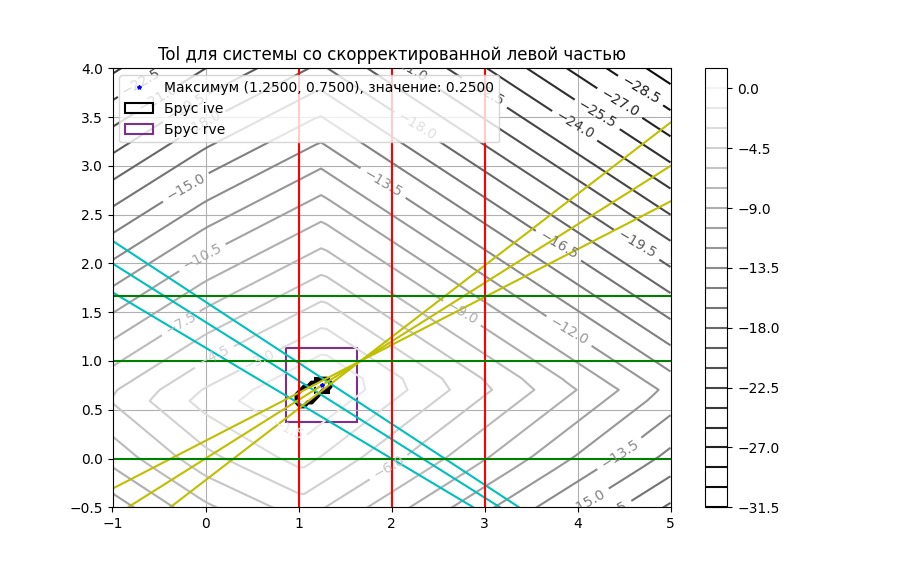
\includegraphics[width=0.7\textwidth]{../src/pic/left.png}
		\caption{Допусковое множество решений со скоректированной матрицей} 
	\end{figure}
	\noindent На данном рисунке черный квадрат имеет сторону $2\cdot \mathrm{ive}$, а фиолетовый - $2\cdot \mathrm{rve}. $ Область обведенная черной линией - допусковое множество\\
	$\mathrm{ive}: 0.068321425 \;\;\;\mathrm{rve}: 0.3444088$
	\begin{figure}[H] \label{MatrixCorrSet}
		\centering
		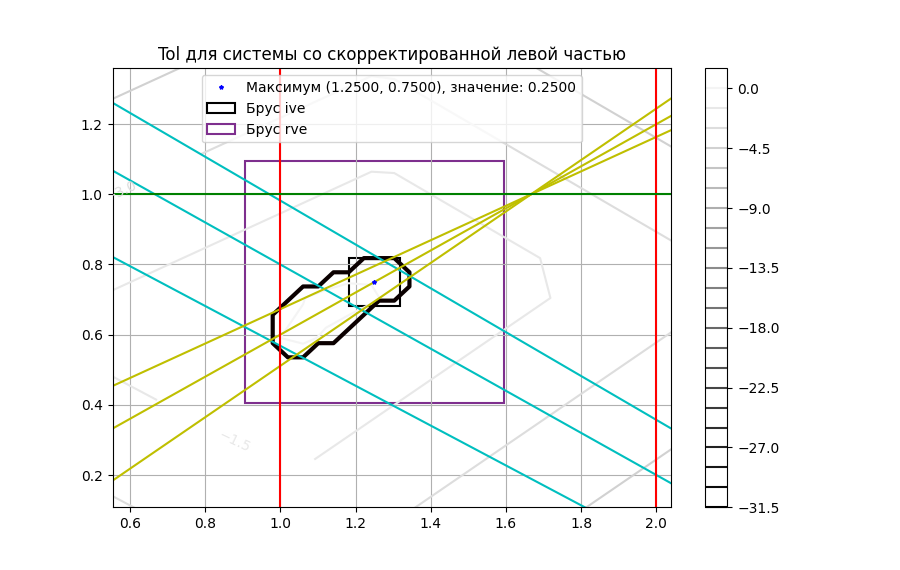
\includegraphics[width=0.6\textwidth]{../src/pic/left_bliz.png}
		\caption{Допусковое множество решений со скоректированной матрицей} 
	\end{figure}
	
	\section{Сравнение}
	\begin{center}
		\begin{tabular}{|c|c|c|c|}
			\hline
			Объект преобразования & argmax Tol & max Tol & Способ коррекции \\ \hline\hline
			Правая часть & (2.80, 1.40) & 0.45 & Увеличим правой части с коэффициентом K=1.35 \\ \hline
			Матрица & (3.29, 1.68) & 0.10 & Сужение матрицы с коэффициентом K=1.35\\ \hline
			1-ая строка & (2.46, 1.23) & -0.73 & Сведение элементов строки в точечные интервалы \\ \hline
			2-ая строка & (3.40, 1.07) & -0.77 & Сведение элементов строки в точечные интервалы \\ \hline
			3-ая строка & (2.80, 1.40) & -0.73 & Сведение элементов строки в точечные интервалы \\ \hline
			4-ая строка & (2.80, 1.40) & -0.90 & Сведение элементов строки в точечные интервалы \\ \hline
		\end{tabular}
	\end{center}
	
	\section{Выводы}
	\begin{enumerate}
		\item После корекции правой части равномерным уширением вектора $\textbf{b}$ безусловный максимум распознающего функционала $Tol$ составляет 0.667 и находится в точке (1.333, 0.667). Заметим, что форма поверхности распознающего функционала $Tol$ не претерпела изменений.
		\item При неравномерном уширении видно, что форма поверхности и расположение безусловных максимумов распознающего функционала $Tol$ до и после неравномерного уширения вектора $\textbf{b}$ не совпадают.
		\item При сравнении этих коррекций можно утверждать, что неравномерное уширение приводит к меньшим значениям вариабельности по сравнению с равномерным уширением.
		\item На нашем примере стоит отметить, что квадрат $rve$ неэффективно аппроксимирует допусковое множество решений. В то время как квадрат $ive$ практически полностью принадлежит $\Xi_{\mathrm{tol}}$. Это обосновано хорошей обусловленностью матрицы ($\mathrm{cond}(\mathrm{mid},\mathbf{A})=1.638$).
	\end{enumerate}
	
	\newpage
	\addcontentsline{toc}{section}{Литература}
	
	\begin{thebibliography}{4}
		\bibitem{s:hist}
		Histogram. URL: \url{https://en.wikipedia.org/wiki/Histogram}
		\bibitem{b:probSectMath}
		Вероятностные разделы математики. Учебник для бакалавров технических направлений.//Под ред. Максимова Ю.Д. --- Спб.: «Иван Федоров», 2001. --- 592 c., илл.
		\bibitem{s:boxplot}
		Box plot. URL: \url{https://en.wikipedia.org/wiki/Box_plot}
		\bibitem{a:nonParamRegr}
		Анатольев, Станислав (2009) «Непараметрическая регрессия», Квантиль, №7, стр. 37-52.
	\end{thebibliography}
	
\end{document}